\chapter{Architettura software}


\section{Architettura generale}

Il progetto è stato realizzato seguendo un'architettura software client-server (figura \ref{fig:arch}). In questa architettura i componenti principali sono: il client rappresentato dall'applicazione iPad oggetto di questo documento, e il lato server scomposto in \emph{middleware} e i sistemi messi a disposizione dal cliente (l'istituto bancario).

Il middleware opera da intermediario tra i servizi bancari e l'applicazione. Tale componente ha il compito di ricevere le richieste dal client, di sottomettere a sua volta queste richieste ai servizi lato banca e di ritornare i dati al client opportunamente formattati.

Le richieste verso il middleware (ospitante un webserver \emph{Apache}) vengono eseguite seguendo un'architettura \emph{RESTFULL}  che prevede richieste \emph{HTTP} (POST, GET, PUT, DELETE). Le risposte fornite dal middleware verso il client sono costruite in formato \emph{JSON}.


\begin{figure}[!htbp]
\centering
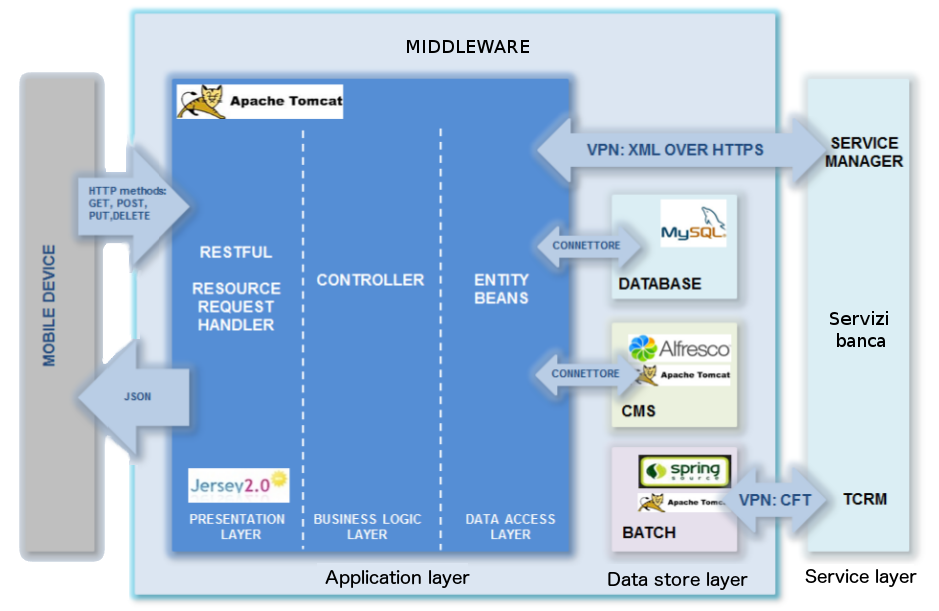
\includegraphics[scale=0.60]{architettura/architect.png}
\caption{Architettura client-server}
\label{fig:arch}
\end{figure}


\section{Architettura applicazione}

L'applicazione è stata progettata usando il design pattern \emph{MVC} (Model-View-Controller, figura \ref{fig:mvc}). In tale pattern ogni oggetto dell'applicazione assolve uno dei seguenti ruoli:
\begin{itemize}
 \item Model: gli oggetti di tipo model hanno il compito di incapsulare i dati specifici a un'applicazione e di definire le logiche per modificare e processare tali dati
 \item View: sono gli oggetti dell'applicazione visibili all'utente. Tali oggetti hanno il compito di visualizzare i dati dell'applicazione e di permetterne l'interazione (esempio la modifica)
 \item Controller: è un oggetto che opera da intermediario tra la view e uno o più model dell'applicazione. Tali oggetti hanno quindi la funzione di comunicare i cambiamenti tra le view e i model, e viceversa.
\end{itemize}

L'utilizzo del pattern MVC permette una migliore estensione del codice, di costruire componenti riusabili e migliorare la definizione delle interfacce.

\begin{figure}[!htbp]
\centering
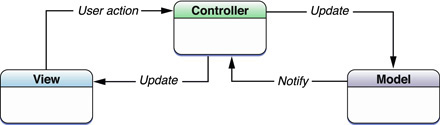
\includegraphics[scale=0.70]{architettura/mvc.png}
\caption{Schema del pattern MVC}
\label{fig:mvc}
\end{figure}

Nei prossimi paragrafi verranno descritte le classi principali del progetto.

\section{Diagramma delle classi}

\subsection{Connessione ai servizi}
\label{parag:networking}
La parte relativa alla gestione delle chiamate ai servizi è stata realizzata implementando delle classi \emph{singleton}. Tali classi estendono la libreria di terze parti \texttt{AFNetworking} che opera da wrapper sulle tecnologie di comunicazione messe a disposizione dall'SDK iOS (Foundation URL Loading System). 

Utilizzare una libreria come AFNetworking ha permesso di ridurre i tempi di sviluppo e di sfruttare le potenzialità offerte dalle sue API come: la serializzazione e deserializzazione dei dati, la possibilità di effettuare richieste HTTP asincrone, una gestione efficiente delle code, la gestione di sessioni, ecc\dots.  

\begin{figure}[!htbp]
\centering
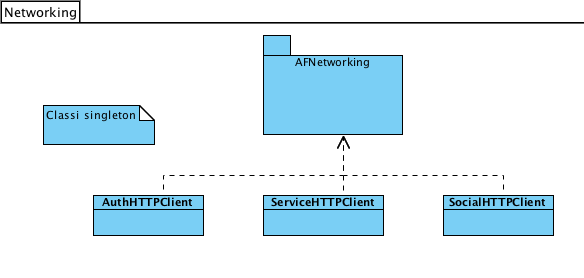
\includegraphics[scale=0.70]{architettura/networkingClass.png}
\caption{Diagramma delle classi per le connessioni di rete}
\end{figure}

% i servizi sono separati da quelli di autenticazione perchè gli  standard oauth richiedono la separazione i sottodimini diversi.

\subsection{Caching dei dati}
Per migliorare le prestazioni e limitare il traffico di rete generato durante l'utilizzo dell'applicazione è stato implementato un meccanismo di caching dei dati che consente di salvare in memoria primaria i dati necessari all'applicazione durante una sessione di utilizzo. 

\begin{figure}[!htbp]
\centering
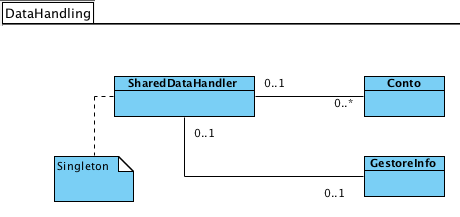
\includegraphics[scale=0.70]{architettura/cacheClass.png}
\caption{Diagramma delle classi per il caching dei dati}
\end{figure}

\subsection{Autenticazione e sicurezza dei dati}
L'applicazione prevede un sistema di autenticazione ai servizi basata su livelli. In particolare sono previsti tre livelli di autenticazione:
\begin{itemize}
 \item autenticazione di livello zero: è il livello associato a un utente che non ha ancora effettuato il login
 \item autenticazione di primo livello: è il livello associato ad un utente che ha precedentemente effettuato il login, ha scelto di ricordare le credenziali e che ha momentaneamente sospeso l'utilizzo dell'applicazione. Questo livello permette all'utente di accedere a un gruppo ristretto di funzionalità nel momento in cui riprenderà l'utilizzo dell'applicazione
 \item autenticazione di secondo livello: è il livello associato ad un utente che ha precedentemente effettuato il login e che permette l'accesso a tutte le funzionalità previste dall'applicazione. Questo livello permane fino a quando l'utente non richiede esplicitamente il logout o sospende l'applicazione
\end{itemize}

\begin{figure}[!htbp]
\centering
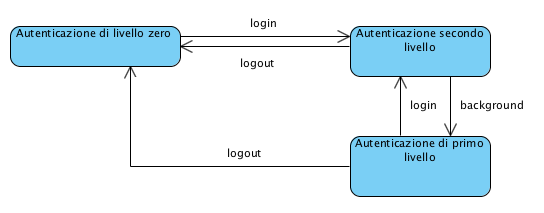
\includegraphics[scale=0.70]{architettura/stati.png}
\caption{Diagramma degli stati di autenticazione}
\end{figure}


L'autenticazione ai servizi è a carico delle classi descritte nel paragrafo \ref{parag:networking}. Questa operazione restituisce in output i dati confidenziali dell'utente che saranno gestiti dalle classi adibite alla sicurezza.

A tal fine è stato implementato un oggetto singleton, il \texttt{SecurityManager}, che ha la responsabilità di stabilire il livello di autenticazione in risposta agli eventi che occorrono all'interno dell'applicazione e di gestire il salvataggio e il recupero dei dati confidenziali dell'utente (come le informazioni sul token, sul numero utente, ecc\dots). Tale classe utilizza la libreria di terze parti \texttt{JNKeychain} che estende le funzioni messe a disposizione dell'SDK iOS, in particolare quelle relative al \emph{Keychain}. 

\begin{figure}[!htbp]
\centering
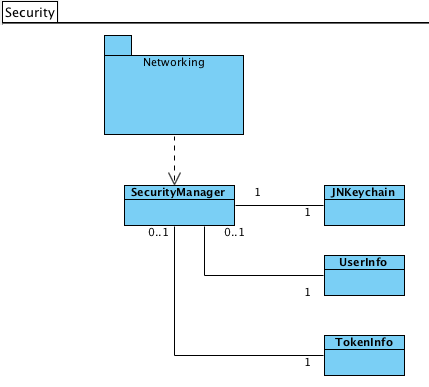
\includegraphics[scale=0.70]{architettura/securityClass.png}
\caption{Diagramma delle classi relative alla sicurezza}
\end{figure}

\subsection{Controller principali}
Di seguito è riportato il diagramma delle classi rappresentanti i controller principali creati durante la progettazione e lo sviluppo. Per semplicità di esposizione sono stati rappresentati solo i nomi dei controller e le relazioni tra essi.
\newline

A titolo esemplificativo nel diagramma si può notare che il \texttt{BaseViewController} è il controller principale dal quale gli altri controller ereditano le funzionalità e proprietà generiche. Tale controller si occupa della creazione e visualizzazione degli  elementi grafici comuni a tutte le interfacce (ad esempio la navigation bar personalizzata) e delle logiche necessarie ad ogni controller che lo specializza.

In particolare uno dei compiti principali di questo controller è quello di creare il controller che gestisce l'interfaccia e la logica per il login ai servizi (\texttt{LoginViewController}) e di implementare il protocollo \texttt{LoginViewControllerProtocol} dichiarato dallo stesso LoginViewController. Sarà quindi compito del LoginViewController  lanciare il processo di login e comunicare al BaseViewController l'esito dell'operazione attraverso il protocollo descritto precedentemente; così facendo il BaseViewController sarà in grado di effettuare l'aggiornamento dello stato dell'interfaccia.


\newpage
\begin{landscape}
\begin{figure}[!htbp]
\centering
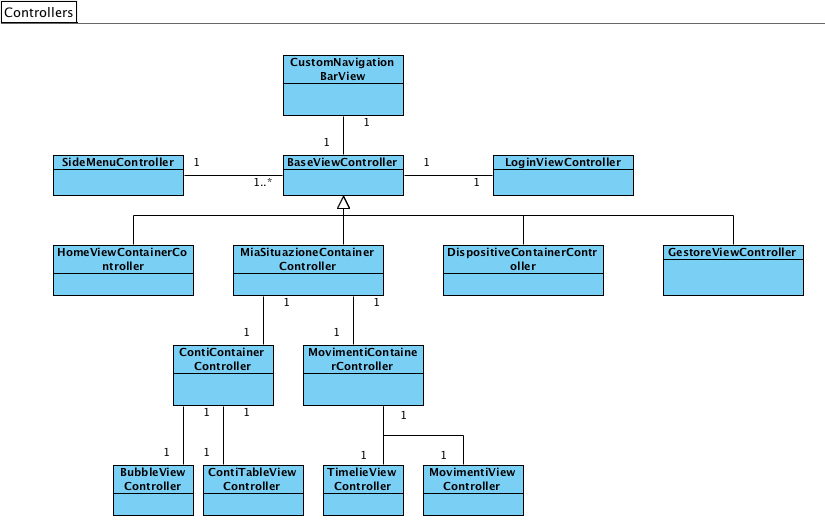
\includegraphics[scale=0.70]{architettura/controllersClass.png}
\caption{Diagramma delle classi controller}
\end{figure}
\end{landscape}
